% Preamble
\documentclass{article}
\usepackage[left=1in, right=1in, top=1in, bottom=1in]{geometry}

% packages
\usepackage {lmodern}
\usepackage [T1]{fontenc}
\usepackage {amsmath}
\usepackage {amssymb}
\usepackage {amsfonts}
\usepackage {graphicx}
\usepackage {fullpage}
\usepackage {gensymb}
\usepackage {caption}
%\usepackage{nopageno}
\usepackage {cite}
\usepackage {setspace}
\usepackage [version=4]{mhchem}
\usepackage{multicol} 
\usepackage{sectsty}

% graphics path
\graphicspath {{images/}}

% bibliography style 
\bibliographystyle{unsrt}    

% font settings
	%%% headings font
	\sectionfont{\fontfamily{ptm}\fontsize{12}{15}\selectfont} 
	\subsectionfont{\fontfamily{ptm}\fontsize{10}{12}\selectfont}

	%%% paragraph font
	\usepackage{fontspec}
	\defaultfontfeatures{Mapping=tex-text, Scale=MatchLowercase}
	\setmainfont{Arial}

% Title
\title{Gas Chromatography \\Analysis of Recreational Alcohol}

\author{{Justin Chao*, Stephen Tung, and Luis Urbiola-Machado}\\[2ex]
The University of Texas at Austin \\ 
justin\_chao@utexas.edu \\ \\
November 4, 2016}
\date{}

% Begin Document
\begin{document}
\maketitle
\unskip\vspace{1.5\baselineskip}


\begin{multicols}{2}

{\fontsize{9.5}{12}\selectfont   

\section*{Abstract}
Alcoholic components of a Cluny scotch whiskey were identified and
quantified using gas chromatography and a flame ionization detector.  The
components identified are as follows: 1-propanol (400 ppm $\pm$
0), ethyl acetate (40 ppm $\pm$ 0), isobutanol
(200 ppm $\pm$ 0), 1-butanol (500 ppm $\pm$ 0), isoamyl
alcohol (100 ppm $\pm$ 0), active amyl alcohol
(40 ppm $\pm$ 0). These findings are determined to be reasonable and
precise.

\section*{Introduction}
This experiment aims to identify and quantify the alcoholic components of a recreational
alcohol using gas chromatography (GC). Chromatography is a technique for
    separating mixtures in a sample. \cite{lab_man}

\subsection*{Gas Chromatography}
Gas Chromatography is a type of chromatography that is used to separate and
    analyze components of a sample by vaporizing them. The mobile phase is
    usually an inert carrier gas such as helium, and the stationary phase is
    usually an inert liquid or polymer on the inside of the column.
    Figure 1 shows a diagram of a gas chromatograph.
    \begin{center}
        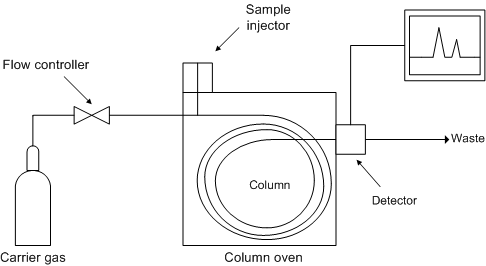
\includegraphics[scale=0.35]{gc.png}
        \captionof{figure}{Diagram of a gas chromatograph.\cite{gc_pic}}
    \end{center}

\subsection*{Flame Ionization Detector}
    A Flame Ionization Detector (FID) quantitatively measures the amount of organic species
in a gaseous sample by detecting the formation of ions during the combustion of
organic compounds in a flame. Figure 2 shows a diagram of an FID.
    \begin{center}
        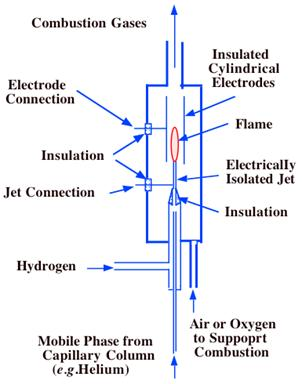
\includegraphics[scale=0.5]{fid.png}
        \captionof{figure}{Diagram of a flame ionization detector.\cite{fid_pic}}
    \end{center}

This method of detection is limited to carbon-hydrogen bond containing compounds, and cannot
detect inorganic substances and highly functionalized species. Furthermore, the
flame used in FID oxidizes any and all oxidizable compounds that pass through
it. FIDs are however, relatively inexpensive to operate, and have very good
linearity and detection ranges. \cite{Harris}

\section*{Experimental}
\subsection*{Instrument Setup}
A Varian 450 GC-FID was used in this experiment with a capillary consisting of
fused silica and CP-SIL 5CB as the coating. The length of the capillary was 60
m, with an internal diameter of 0.25 mm. The temperature was held at
80$\degree$C for 1 min, then ramped to 100$\degree$C at 5$\degree$C/min for
another minute, and finally to 140$\degree$C at 4$\degree$C/min for another
minute.  The injector and detector temperatures were kept at 180$\degree$C.  A
flow rate of 2.4 mL/min was maintained with a mixture of 5.0 ultra-high purity
hydrogen gas at 32 psi, air at 51 psi, and helium at 74 psi as the carrier gas.

\subsection*{Sample Preparation}
A Cluny blended scotch whisky was used as the sample to be analyzed.
All injections were done using the sandwich method.
A chromatograph of 1.0 µL of the whiskey sample was taken as a qualitative
    analysis. 
A 50.0 mL standard solution was prepared, consisting of 25.0 µL of each of the
    following: 1-butanol, 2-methyl-1-propanol, ethyl acetate,
    3-methyl-1-butanol, 2-methyl-1-butanol, and 1-propanol. The solution was
    diluted with 40\% ethanol. Three chromatograph were then taken of the standard
    solution, using 0.5 µL.

A 50.0 mL sample solution was prepared, consisting of 25.0 µL of 1-butanol and
    diluted with the whiskey sample. Three chromatographs were then taken of the
    spiked sample, using 1.0 µL.

\section*{Results}

The concentrations of the components identified are given in Table 1.

  \begin{center} 
      \captionof{table}{Concentrations of identified compounds.}
   \resizebox{0.5\textwidth}{!}{\begin{tabular}{lrrrr}
       \textbf{Alcohol} & \multicolumn{1}{l}{Concentration (ppm)} & \multicolumn{1}{l}{Std Dev} & \multicolumn{1}{l}{RSD} & \multicolumn{1}{l}{90\% CI} \\
       \hline
       1-propanol & 400 & 0 & 0 & 0 \\
       ethyl acetate & 40 & 0 & 0 & 0 \\
       isobutanol & 200 & 0 & 0 & 0 \\
       1-butanol & 500 & 0 & 0 & 0 \\
       isoamyl alcohol & 100 & 0 & 0 & 0 \\
       active amyl alcohol & 40 & 0 & 0 & 0 \\
   \end{tabular}}
  \end{center}


\section*{Discussion}
The results of this experiment given in Table 1 are reasonable and precise.
No reference was available to compare the accuracy of the results with.
Additional measures for improving precision may include the inclusion of more
trials.

[1a] The internal standard standardizes the relative response of the detector to
analyte and sample. This is necessary because sample injection amounts and run
conditions may change with different trials. The internal standard also serves
as a known constant on the chromatograph, and helps to identify other compounds in the
sample based on elute order. 
[1b] The internal standard should be similar to the
analyte and have similar retention times. It should also be stable and not
interfere or react with the sample components. 
[1c] The increased injection volume does not factor into the calculations for
quantifying the alcohol components since the calculations rely on the detector
response factor calculated from the standard solution, and not on the volume of
standard components directly. 
[1d] The purpose of the qualitative whiskey sample is to provide a
reference of elute order for the identification of the components. 
[1e] An internal standard would still be necessary, even if a calibration curve was
constructed, for the determination of the relative response factor of the
detector to analyte and sample.

[2] The purity of the reagents is important due to the high sensitivity,
linearity, and detection of GC.

[3] Capillary columns, against packed columns, have larger theoretical plate
numbers, high resolution, and excel at analysis of low concentrations. The
disadvantages though, include the possibility of overloading the phase.

[4a] A Flame Ionization Detector (FID) quantitatively measures the amount of organic species
in a gaseous sample by detecting the formation of ions during the combustion of
organic compounds in a flame. Figure 2 shows a diagram of an FID.
[4b] A Thermal Conductivity Detector (TCD) detects changes in the thermal
conductivity of the effluent by comparing it to a reference flow of carrier gas.
Most compounds have a thermal conductivity less than that of helium or hydrogen,
the more commonly used carrier gasses. Therefore, when an analyte elutes, the
total thermal conductivity of the effluent is decreased, and this change is
detected by the TCD.
[4c] Both FID and TCD are classified as bulk detectors, because they detect
properties that both the analyte and carrier gas possess, although to different
degrees.
[4d] FID is limited to carbon-hydrogen bond containing compounds, and cannot
detect inorganic substances and highly functionalized species. Furthermore, the
flame used in FID oxidizes any and all oxidizable compounds that pass through
it. FIDs are however, relatively inexpensive to operate, and have very good
linearity and detection ranges. \cite{Harris}
Unlike FID, TCD responds to all compounds and therefore is a good general
purpose detector for initial investigations of an unknown sample. The
sensitivity and limit of detection for TCD however, is not as good as FID.

[5a] A mass spectrometer can also be used as a GC detector. As molecules elute
from the column at different times, the mass spectrometer breaks each molecule
into ionized fragments, and then detects these fragments using their
mass-to-charge ratio.
[5b] The mass spectrum produced from a mass spectrometer may be used to determine
isotopic signatures of a sample, masses of particles and molecules, and the
chemical structures of compounds.
[5c] A FID may not be able to differentiate between multiple components that
happen to have similar retention times. Mass spectrometry however, is able to
differentiate between co-elutes. Disadvantages of this method however, include
the inability to distinguish between geometrical and optical isomers. The scope
of mass spectrometry is also limited in identifying hydrocarbons that fragment
into similar ions.

[6a] The effects of linear flow rate on the height equivalent of a theoretical
plate in separation can be described by the van Deemter equation. In gas
chromatography with an open tubular column, the B term has the largest effect on
the separation efficiency, representing the longitudinal diffusion or natural
diffusion tendency of molecules. The A term is equal to 0 for an open tubular column,
and the C term.
[6b] Figure 3 shows a sketch of a qualitative van Deemter plot for this experiment.
\begin{center}
    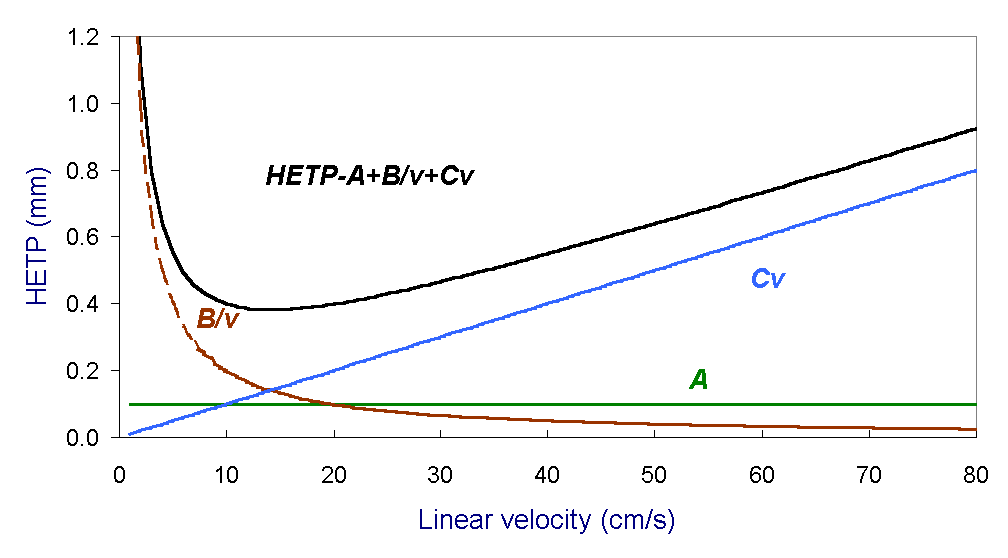
\includegraphics[scale=0.2]{HETP.png}
    \captionof{figure}{Qualitative sketch of a van Deemter plot.\cite{usu}}
\end{center}
[6c] Physical parameters that can be adjusted to increase the efficiency of GC
separation include increasing pressure and temperature while decreasing column
diameter and increasing column length.
[6d] Increasing column length would result in longer retention times and longer
run times. However, this can be mitigated if the column diameter were to be decreased and the pressure
and temperature increased, keeping run times in reasonable domain.

\subsection*{Literature Review}
Another experiment that utilizes GC-FID can be found in the article:
"Application of specific response factors in the gas chromatographic analysis of
methyl esters of fatty acids with flame ionization detectors".\cite{ref}
The carrier gas used in this article was a mixture of hydrogen at 40 mL/min and air at 400
mL/min, and argon at 10 psi. No internal standard was given.

\section*{Conclusion}
Boiling point comparison may be used to theoretically determine the elution
order of compounds in gas chromatography. Compounds with lower boiling points
should elute earlier than those with higher boiling points, and this is seen to
be the case in the data gathered for this experiment. The only exception is the
elution order of isoamyl alcohol and active amyl alcohol, where isoamyl alcohol
alcohol elutes first despite having a slightly higher boiling point than active
amyl alcohol. While the difference is slight, this reversed order of elution may
be due to difference in affinity towards the stationary phase. In other words,
active amyl alcohol may be more attracted to the stationary phase than isoamyl
alcohol, resulting in longer retention times.

The results of this experiment are found to be reasonable, precise, and reproducible. There
were no references to compare the accuracy of the results with.

Possible sources of error in this experiment include random errors in the
preparation of chemicals and samples to be analyzed, as multiple people were
involved in the samples preparation. This may cause discrepancies in the
retention times and sample concentrations found for each compound.

Possible areas for improving the experiment may include the adjustment of column
and physical parameters to improve the efficiency of gas chromatography as
discussed in the discussion section above.


\bibliography{GC-FID.bib}

}
\end{multicols}



\newpage
\section*{Appendix}
\begin{enumerate}
    \item Raw data of tables and chromatograms.
    \item Table of standard retention times.
    \item Table of standard peak areas.
    \item Table of detector response factors.
    \item Table of calculated alcohol component concentrations.
    \item Table of sample peak widths 50\%.
    \item Table of sample retention times.
    \item Table of number of theoretical plates.
    \item Table of heigh equivalent to a theoretical plate.
    \item Sample calculations for the concentration of 1-propanol.
    \item Laboratory notebook copies.
\end{enumerate}
\newpage

\begin{center}

	% Whiskey Qualitative
    \captionof{table}{Qualitative whiskey chromatogram run.}
   \resizebox{0.9\textwidth}{!}{\begin{tabular}{lrrrrrrr}
   \textbf{Whiskey} & \multicolumn{1}{l}{\textbf{Qualitative}} &   &   &   &   &   &  \\
   \# & \multicolumn{1}{l}{Name} & \multicolumn{1}{l}{Time [Min]} & \multicolumn{1}{l}{Quantity [\% Area]} & \multicolumn{1}{l}{Height [µV]} & \multicolumn{1}{l}{Area [µV.Min]} & \multicolumn{1}{l}{Area \% [\%]} & \multicolumn{1}{l}{Width 50\% [Min]} \\
       \hline
   \multicolumn{1}{r}{1} & \multicolumn{1}{l}{1-proponal} & 3.61 & 54.26 & 103470.9 & 1869.6 & 54.264 & 0.016 \\
   \multicolumn{1}{r}{2} & \multicolumn{1}{l}{ethyl acetate} & 3.89 & 0.94 & 2102.2 & 32.4 & 0.941 & 0.015 \\
   \multicolumn{1}{r}{3} & \multicolumn{1}{l}{isobutanol} & 3.98 & 2.83 & 5703 & 97.5 & 2.83 & 0.017 \\
   \multicolumn{1}{r}{4} & \multicolumn{1}{l}{1-butanol} & 4.12 & 22.88 & 39933.3 & 788.4 & 22.884 & 0.018 \\
   \multicolumn{1}{r}{5} & \multicolumn{1}{l}{isoamyl alcohol} & 5.41 & 14.33 & 18640.3 & 493.7 & 14.33 & 0.024 \\
   \multicolumn{1}{r}{6} & \multicolumn{1}{l}{active amyl alcohol} & 5.48 & 4.75 & 6609.6 & 163.7 & 4.752 & 0.024 \\
     &   &   &   &   &   &   &  \\
   Total &   &   & 100 & 176459.3 & 3445.4 & 100 &  \\
   \end{tabular}}

    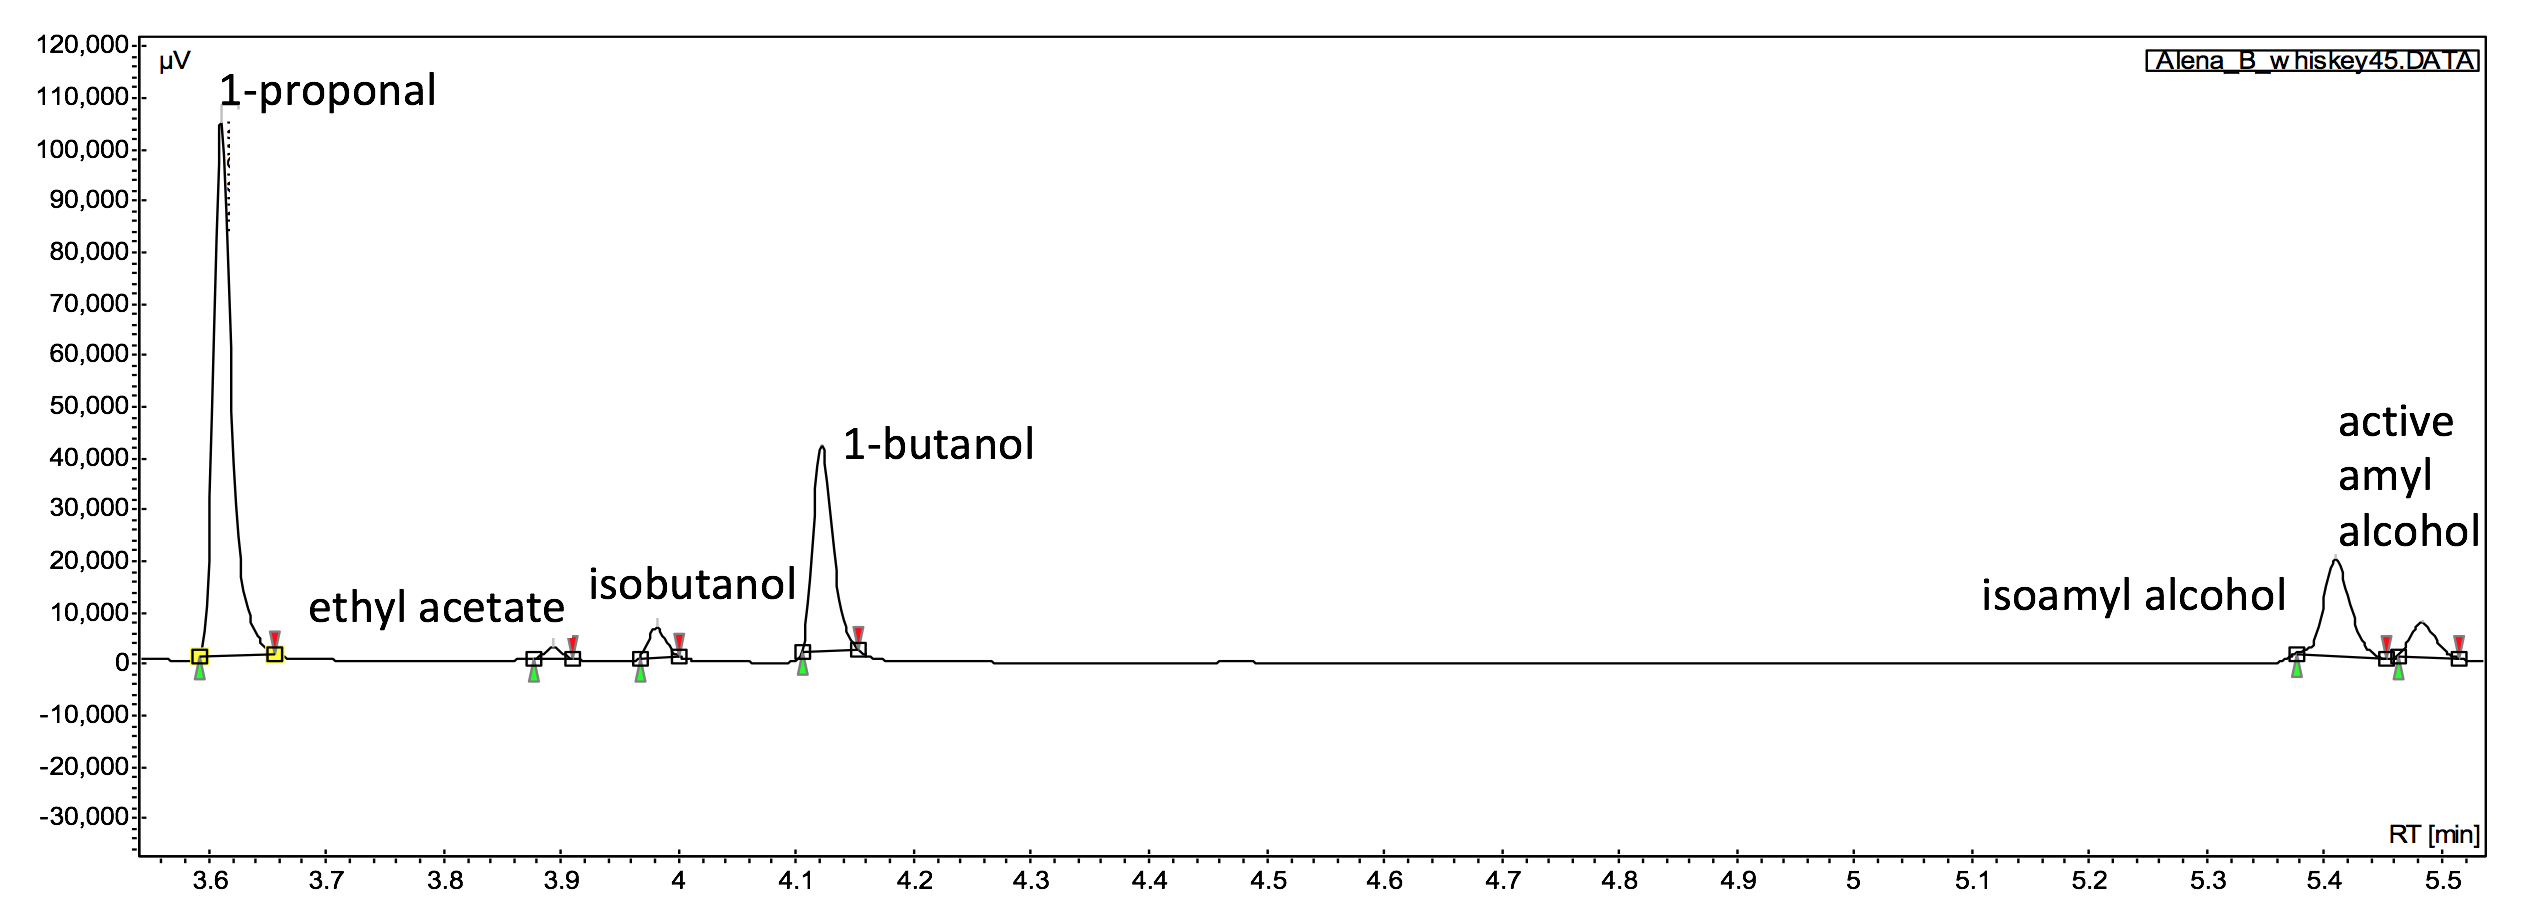
\includegraphics[scale=0.3]{whiskey.png}
    \captionof{figure}{Chromatogram of qualitative whiskey sample run.}

\vspace{1cm}

	% Standard_1
    \captionof{table}{Standard chromatogram run 1.}
   \resizebox{0.9\textwidth}{!}{\begin{tabular}{lrrrrrrr}
   \textbf{Standard\_1} &   &   &   &   &   &   &  \\
   \# & \multicolumn{1}{l}{Name} & \multicolumn{1}{l}{Time [Min]} & \multicolumn{1}{l}{Quantity [\% Area]} & \multicolumn{1}{l}{Height [µV]} & \multicolumn{1}{l}{Area [µV.Min]} & \multicolumn{1}{l}{Area \% [\%]} & \multicolumn{1}{l}{Width 50\% [Min]} \\
       \hline
   \multicolumn{1}{r}{1} & \multicolumn{1}{l}{1-proponal} & 3.6 & 16.95 & 48038.4 & 1108.3 & 16.951 & 0.021 \\
   \multicolumn{1}{r}{2} & \multicolumn{1}{l}{ethyl acetate} & 3.97 & 11.76 & 31686.6 & 769.1 & 11.763 & 0.023 \\
   \multicolumn{1}{r}{3} & \multicolumn{1}{l}{isobutanol} & 4.11 & 18.2 & 49231.8 & 1189.9 & 18.199 & 0.022 \\
   \multicolumn{1}{r}{4} & \multicolumn{1}{l}{1-butanol} & 4.45 & 19.84 & 51127.7 & 1297.4 & 19.844 & 0.023 \\
   \multicolumn{1}{r}{5} & \multicolumn{1}{l}{isoamyl alcohol} & 5.39 & 18.23 & 43394.7 & 1192.2 & 18.234 & 0.026 \\
   \multicolumn{1}{r}{6} & \multicolumn{1}{l}{active amyl alcohol} & 5.47 & 15.01 & 35454.4 & 981.4 & 15.01 & 0.026 \\
     &   &   &   &   &   &   &  \\
   Total &   &   & 100 & 258933.6 & 6538.2 & 100 &  \\
   \end{tabular}}

    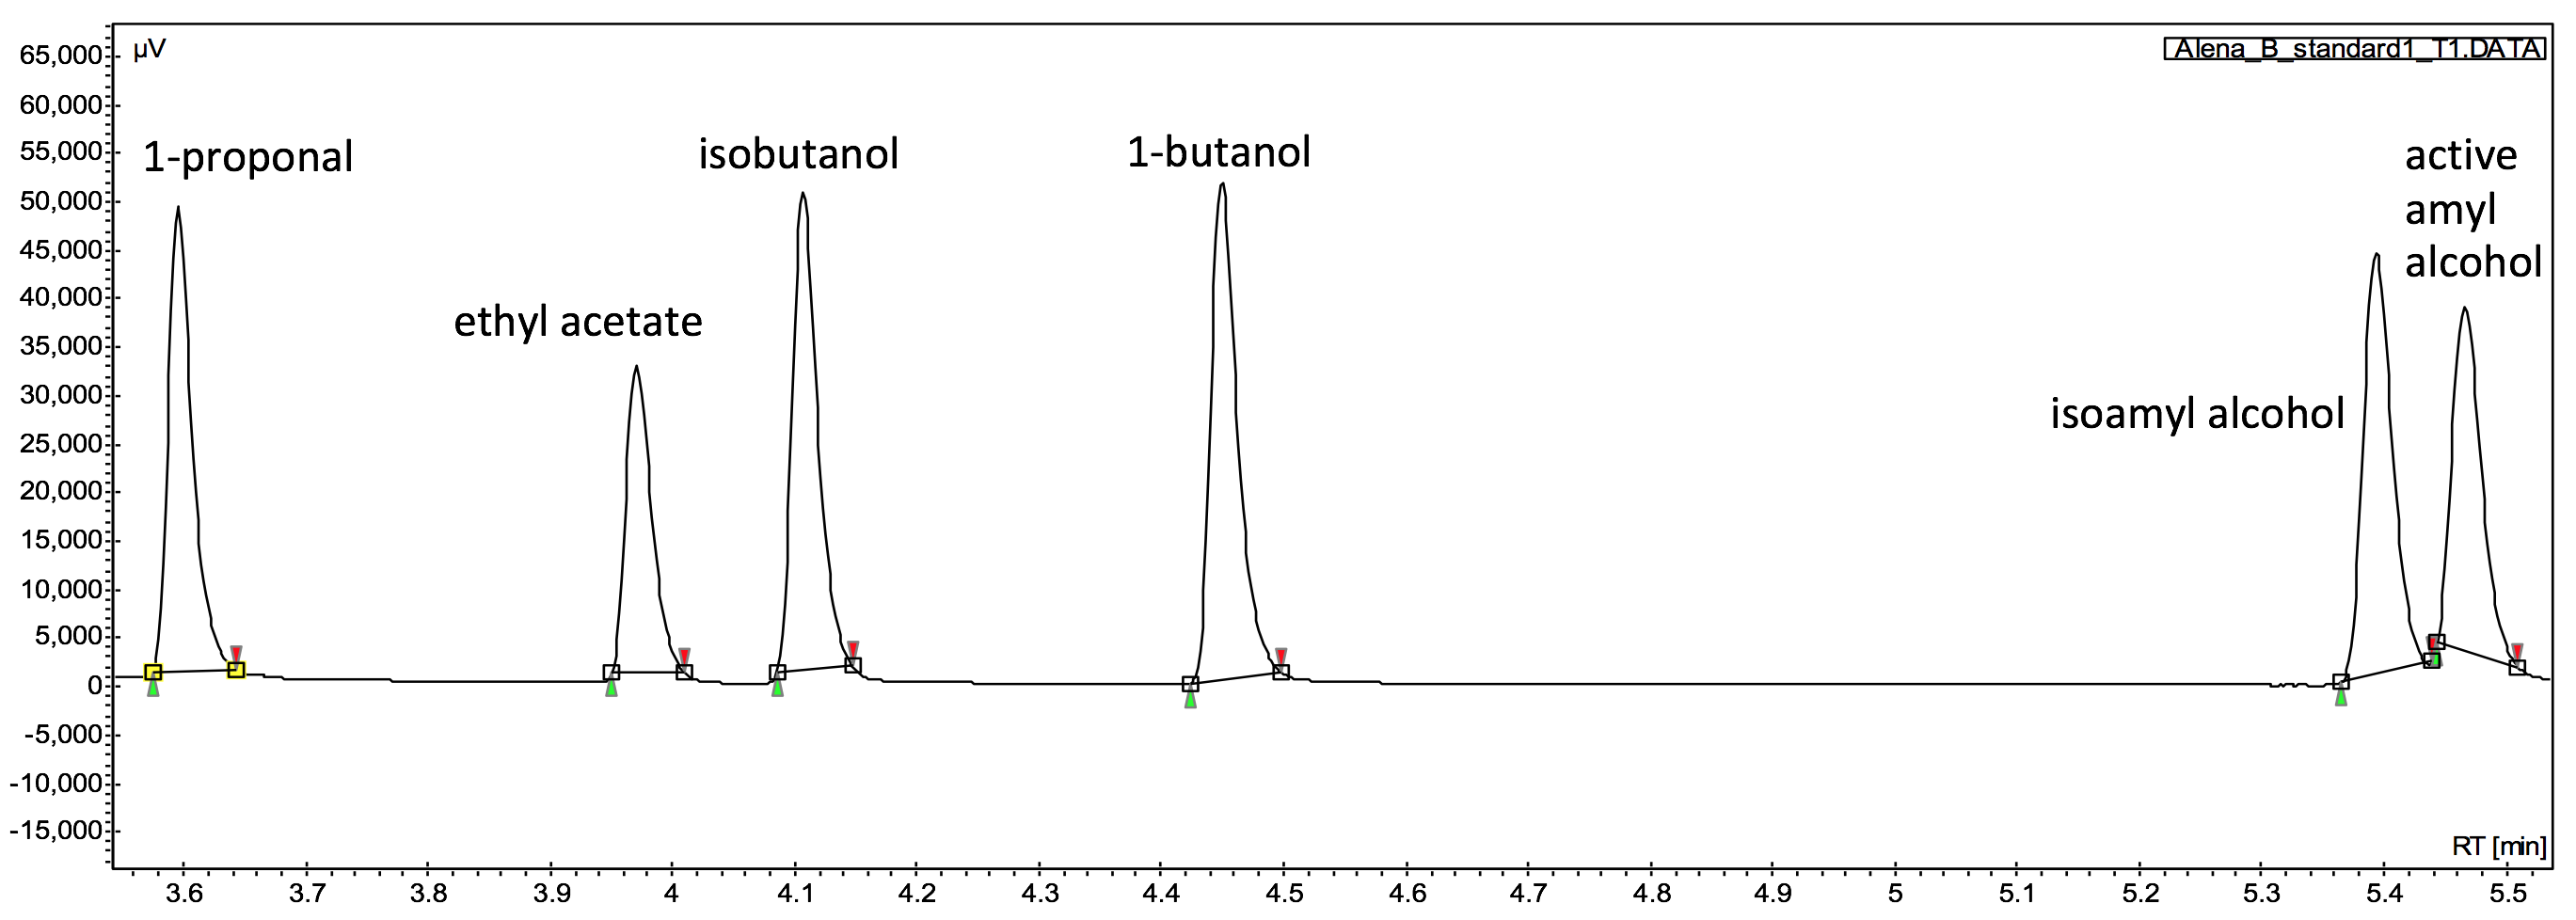
\includegraphics[scale=0.3]{standard1.png}
    \captionof{figure}{Chromatogram of standard sample run 1.}

	% Standard_2
    \captionof{table}{Standard chromatogram run 2.}
   \resizebox{0.9\textwidth}{!}{\begin{tabular}{lrrrrrrr}
   \textbf{Standard\_2} &   &   &   &   &   &   &  \\
   \# & \multicolumn{1}{l}{Name} & \multicolumn{1}{l}{Time [Min]} & \multicolumn{1}{l}{Quantity [\% Area]} & \multicolumn{1}{l}{Height [µV]} & \multicolumn{1}{l}{Area [µV.Min]} & \multicolumn{1}{l}{Area \% [\%]} & \multicolumn{1}{l}{Width 50\% [Min]} \\
       \hline
   \multicolumn{1}{r}{1} & \multicolumn{1}{l}{1-proponal} & 3.6 & 16.56 & 13788.5 & 451.7 & 16.558 & 0.032 \\
   \multicolumn{1}{r}{2} & \multicolumn{1}{l}{ethyl acetate} & 3.98 & 12.55 & 11098.3 & 342.3 & 12.549 & 0.03 \\
   \multicolumn{1}{r}{3} & \multicolumn{1}{l}{isobutanol} & 4.11 & 18.25 & 15733.6 & 497.9 & 18.253 & 0.031 \\
   \multicolumn{1}{r}{4} & \multicolumn{1}{l}{1-butanol} & 4.46 & 19.55 & 16500 & 533.2 & 19.547 & 0.031 \\
   \multicolumn{1}{r}{5} & \multicolumn{1}{l}{isoamyl alcohol} & 5.4 & 17.4 & 15287.6 & 474.6 & 17.4 & 0.03 \\
   \multicolumn{1}{r}{6} & \multicolumn{1}{l}{active amyl alcohol} & 5.47 & 15.69 & 12960.5 & 428.1 & 15.694 & 0.031 \\
     &   &   &   &   &   &   &  \\
   Total &   &   & 100 & 85368.3 & 2727.8 & 100 &  \\
   \end{tabular}}

    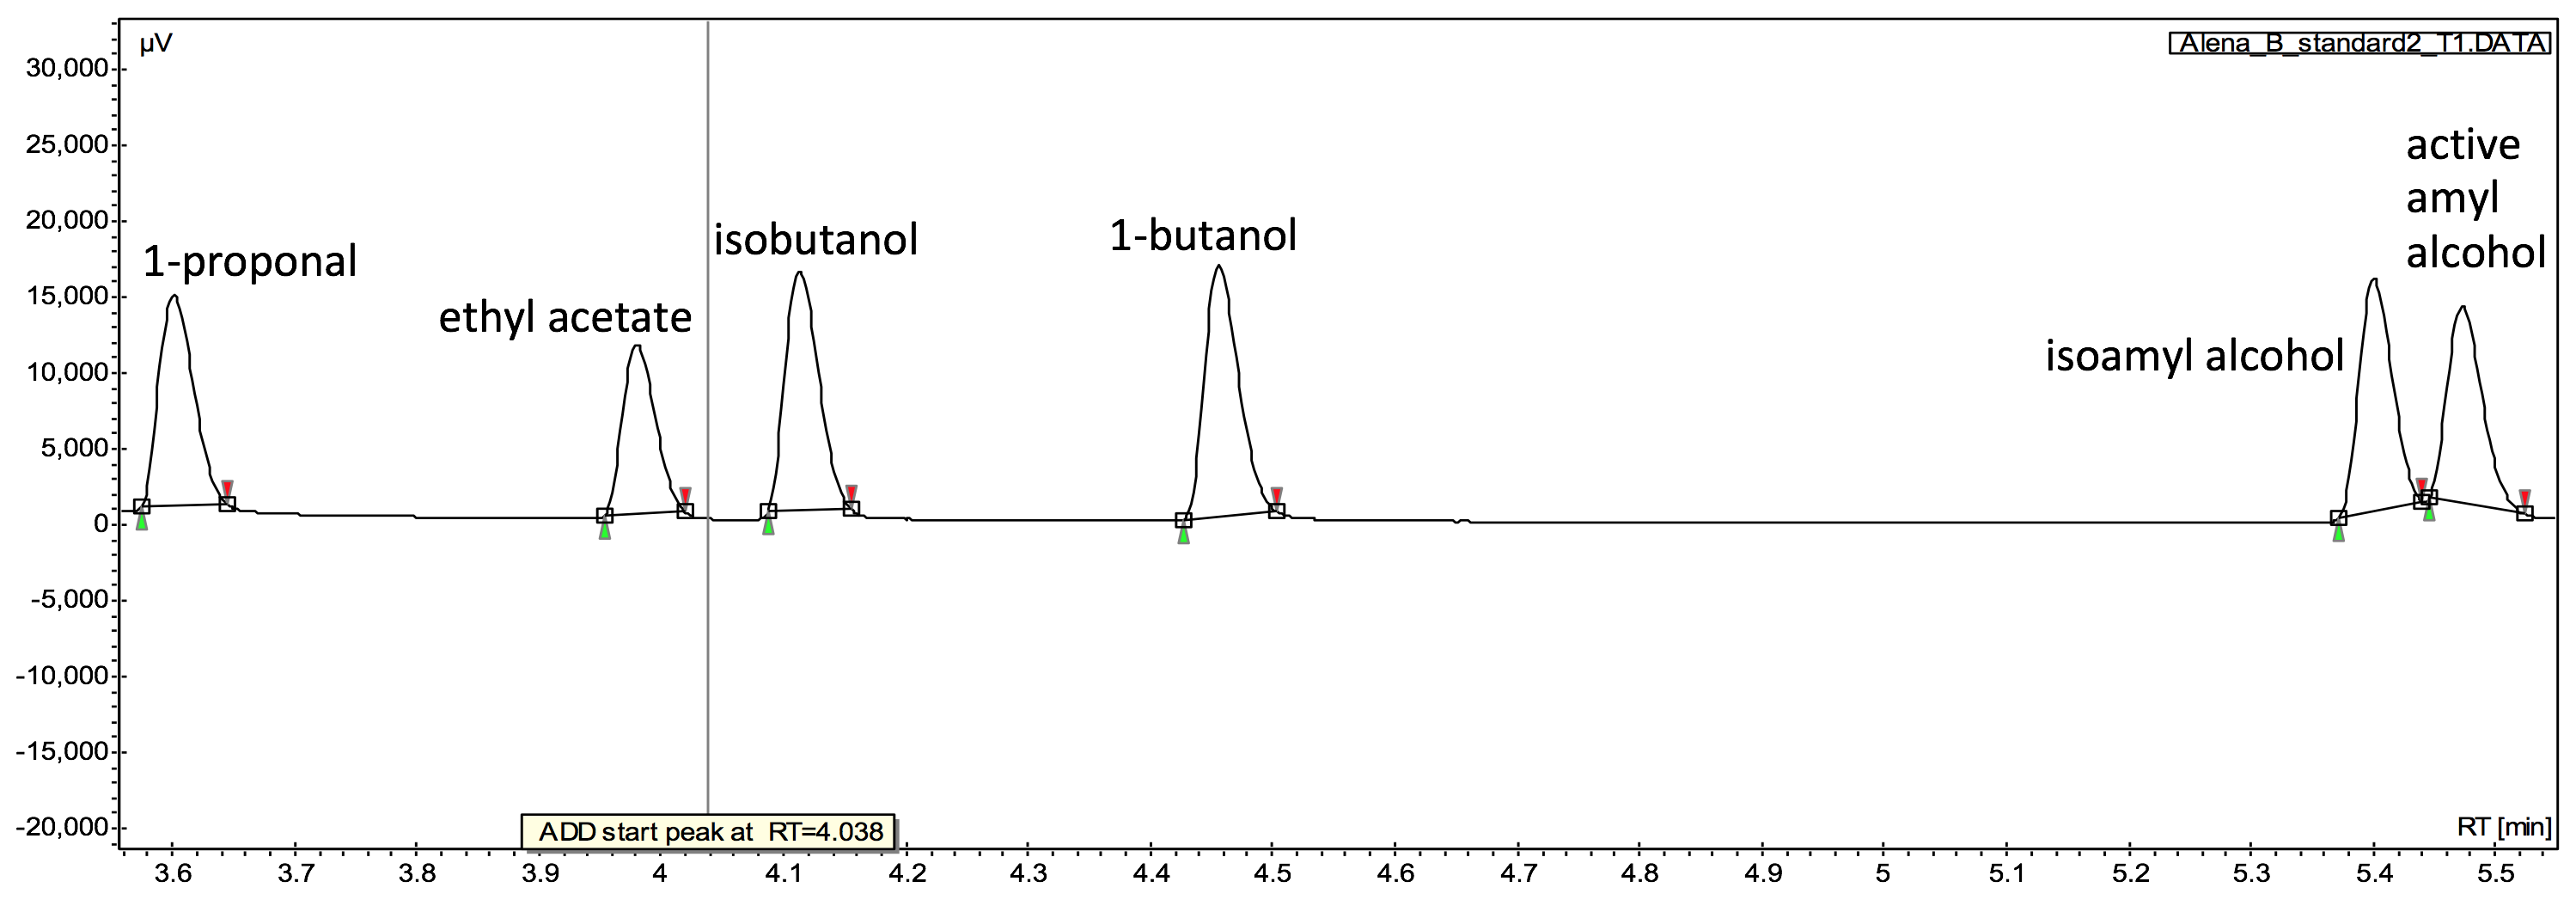
\includegraphics[scale=0.3]{standard2.png}
    \captionof{figure}{Chromatogram of standard sample run 2.}

    \vspace{0.8cm}

	% Standard_3
    \captionof{table}{Standard chromatogram run 3.}
   \resizebox{0.9\textwidth}{!}{\begin{tabular}{lrrrrrrr}
   \textbf{Standard\_3} &   &   &   &   &   &   &  \\
   \# & \multicolumn{1}{l}{Name} & \multicolumn{1}{l}{Time [Min]} & \multicolumn{1}{l}{Quantity [\% Area]} & \multicolumn{1}{l}{Height [µV]} & \multicolumn{1}{l}{Area [µV.Min]} & \multicolumn{1}{l}{Area \% [\%]} & \multicolumn{1}{l}{Width 50\% [Min]} \\
       \hline
   \multicolumn{1}{r}{1} & \multicolumn{1}{l}{1-proponal} & 3.6 & 16.4 & 31063 & 870.3 & 16.399 & 0.026 \\
   \multicolumn{1}{r}{2} & \multicolumn{1}{l}{ethyl acetate} & 3.98 & 11.5 & 20808.6 & 610.1 & 11.496 & 0.027 \\
   \multicolumn{1}{r}{3} & \multicolumn{1}{l}{isobutanol} & 4.11 & 18.61 & 34118.6 & 987.8 & 18.613 & 0.027 \\
   \multicolumn{1}{r}{4} & \multicolumn{1}{l}{1-butanol} & 4.45 & 20.29 & 36516.7 & 1076.7 & 20.289 & 0.027 \\
   \multicolumn{1}{r}{5} & \multicolumn{1}{l}{isoamyl alcohol} & 5.4 & 17.89 & 32154.5 & 949.6 & 17.893 & 0.028 \\
   \multicolumn{1}{r}{6} & \multicolumn{1}{l}{active amyl alcohol} & 5.47 & 15.31 & 26796.5 & 812.5 & 15.31 & 0.028 \\
     &   &   &   &   &   &   &  \\
   Total &   &   & 100 & 181457.8 & 5306.8 & 100 &  \\
   \end{tabular}}

    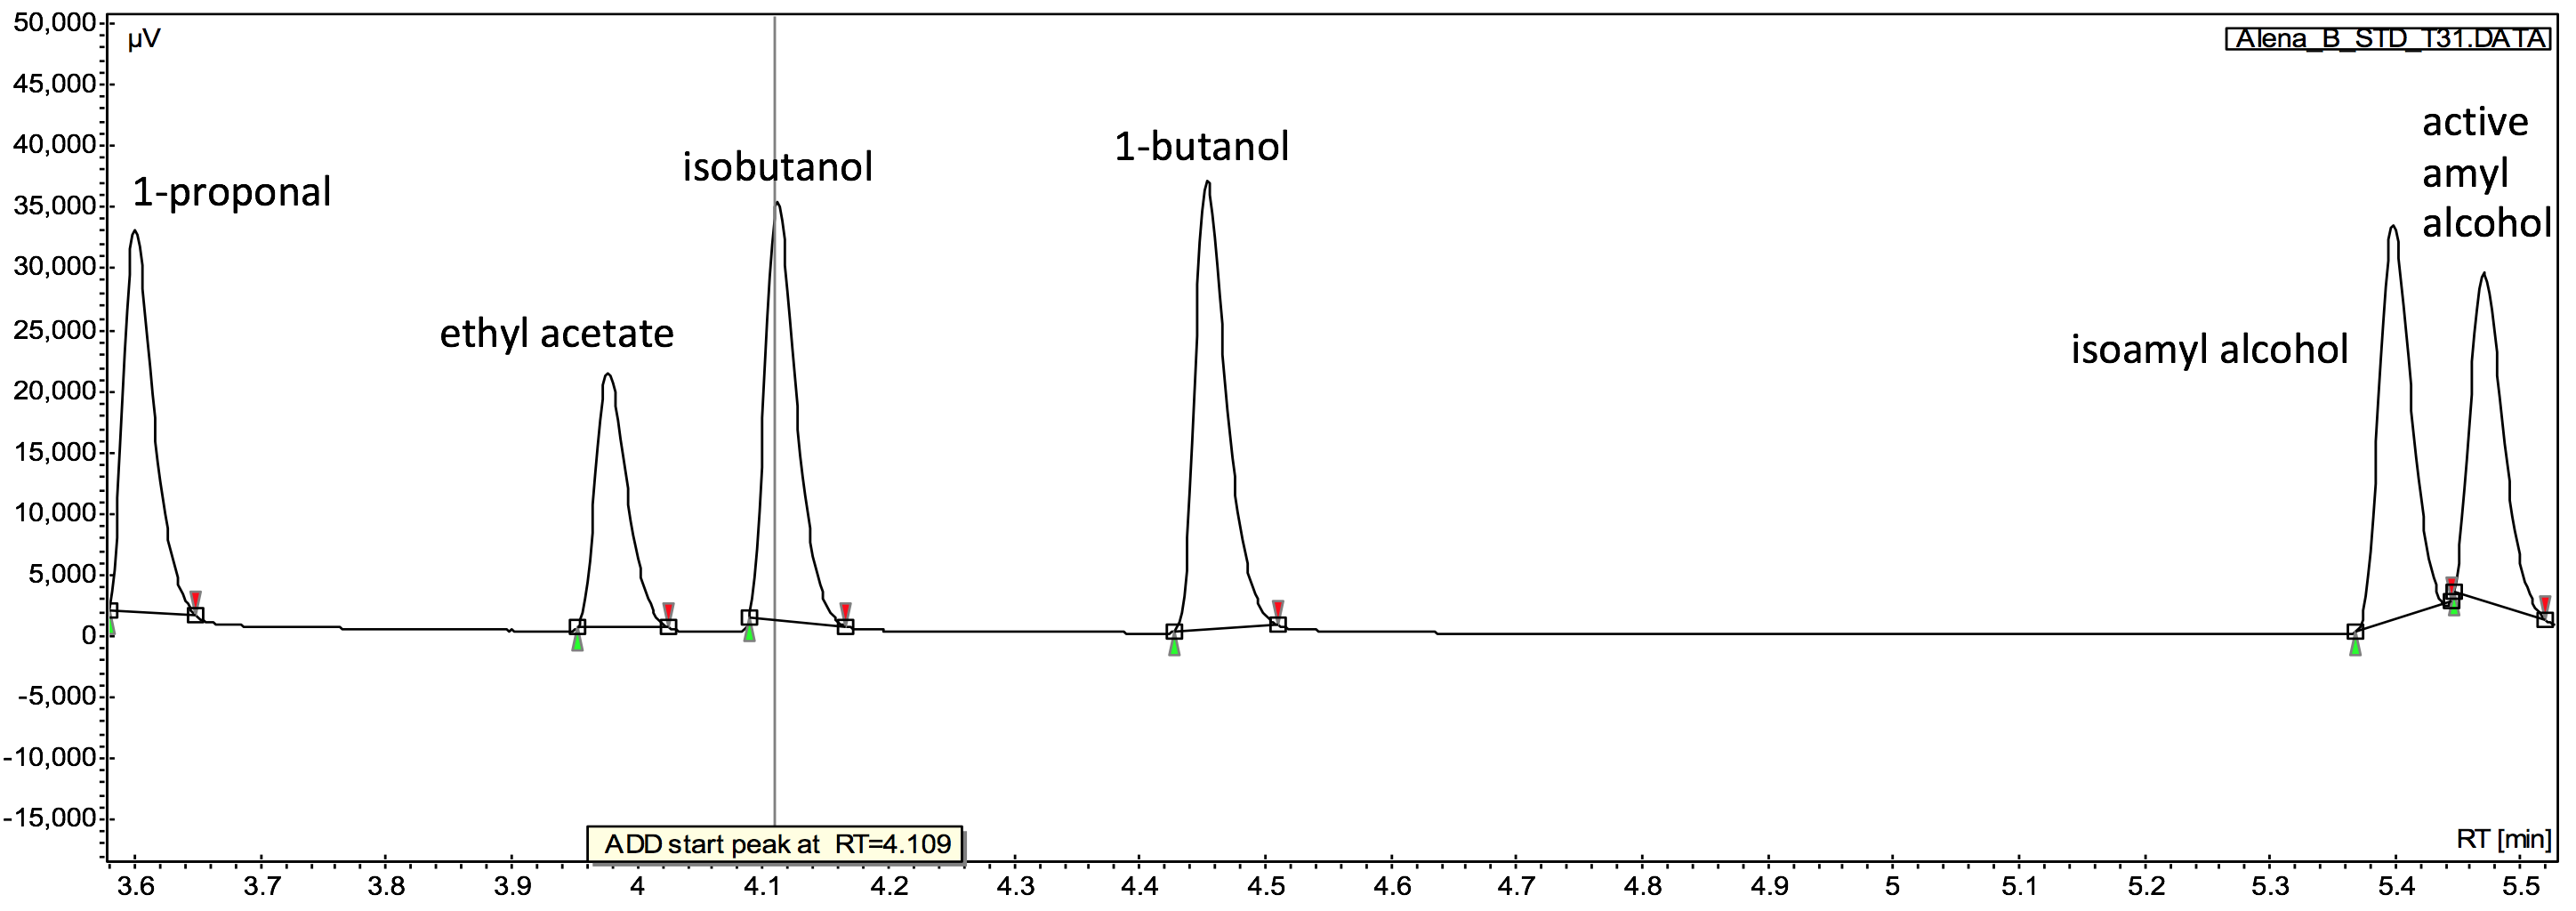
\includegraphics[scale=0.3]{standard3.png}
    \captionof{figure}{Chromatogram of standard sample run 3.}

	% Sample_1
    \captionof{table}{Whiskey sample chromatogram run 1}
   \resizebox{0.9\textwidth}{!}{\begin{tabular}{lrrrrrrr}
   \textbf{Sample\_1} &   &   &   &   &   &   &  \\
   \# & \multicolumn{1}{l}{Name} & \multicolumn{1}{l}{Time [Min]} & \multicolumn{1}{l}{Quantity [\% Area]} & \multicolumn{1}{l}{Height [µV]} & \multicolumn{1}{l}{Area [µV.Min]} & \multicolumn{1}{l}{Area \% [\%]} & \multicolumn{1}{l}{Width 50\% [Min]} \\
       \hline
   \multicolumn{1}{r}{1} & \multicolumn{1}{l}{1-proponal} & 3.6 & 29.99 & 118621.6 & 1993.2 & 29.992 & 0.015 \\
   \multicolumn{1}{r}{2} & \multicolumn{1}{l}{ethyl acetate} & 3.97 & 1.95 & 7535.5 & 129.3 & 1.946 & 0.017 \\
   \multicolumn{1}{r}{3} & \multicolumn{1}{l}{isobutanol} & 4.11 & 14.7 & 47287.5 & 976.6 & 14.696 & 0.019 \\
   \multicolumn{1}{r}{4} & \multicolumn{1}{l}{1-butanol} & 4.45 & 42.38 & 130357.8 & 2816.8 & 42.385 & 0.019 \\
   \multicolumn{1}{r}{5} & \multicolumn{1}{l}{isoamyl alcohol} & 5.4 & 8.42 & 21047.5 & 559.3 & 8.416 & 0.024 \\
   \multicolumn{1}{r}{6} & \multicolumn{1}{l}{active amyl alcohol} & 5.47 & 2.57 & 7199 & 170.5 & 2.566 & 0.023 \\
     &   &   &   &   &   &   &  \\
   Total &   &   & 100 & 332049 & 6645.8 & 100 &  \\
   \end{tabular}}

    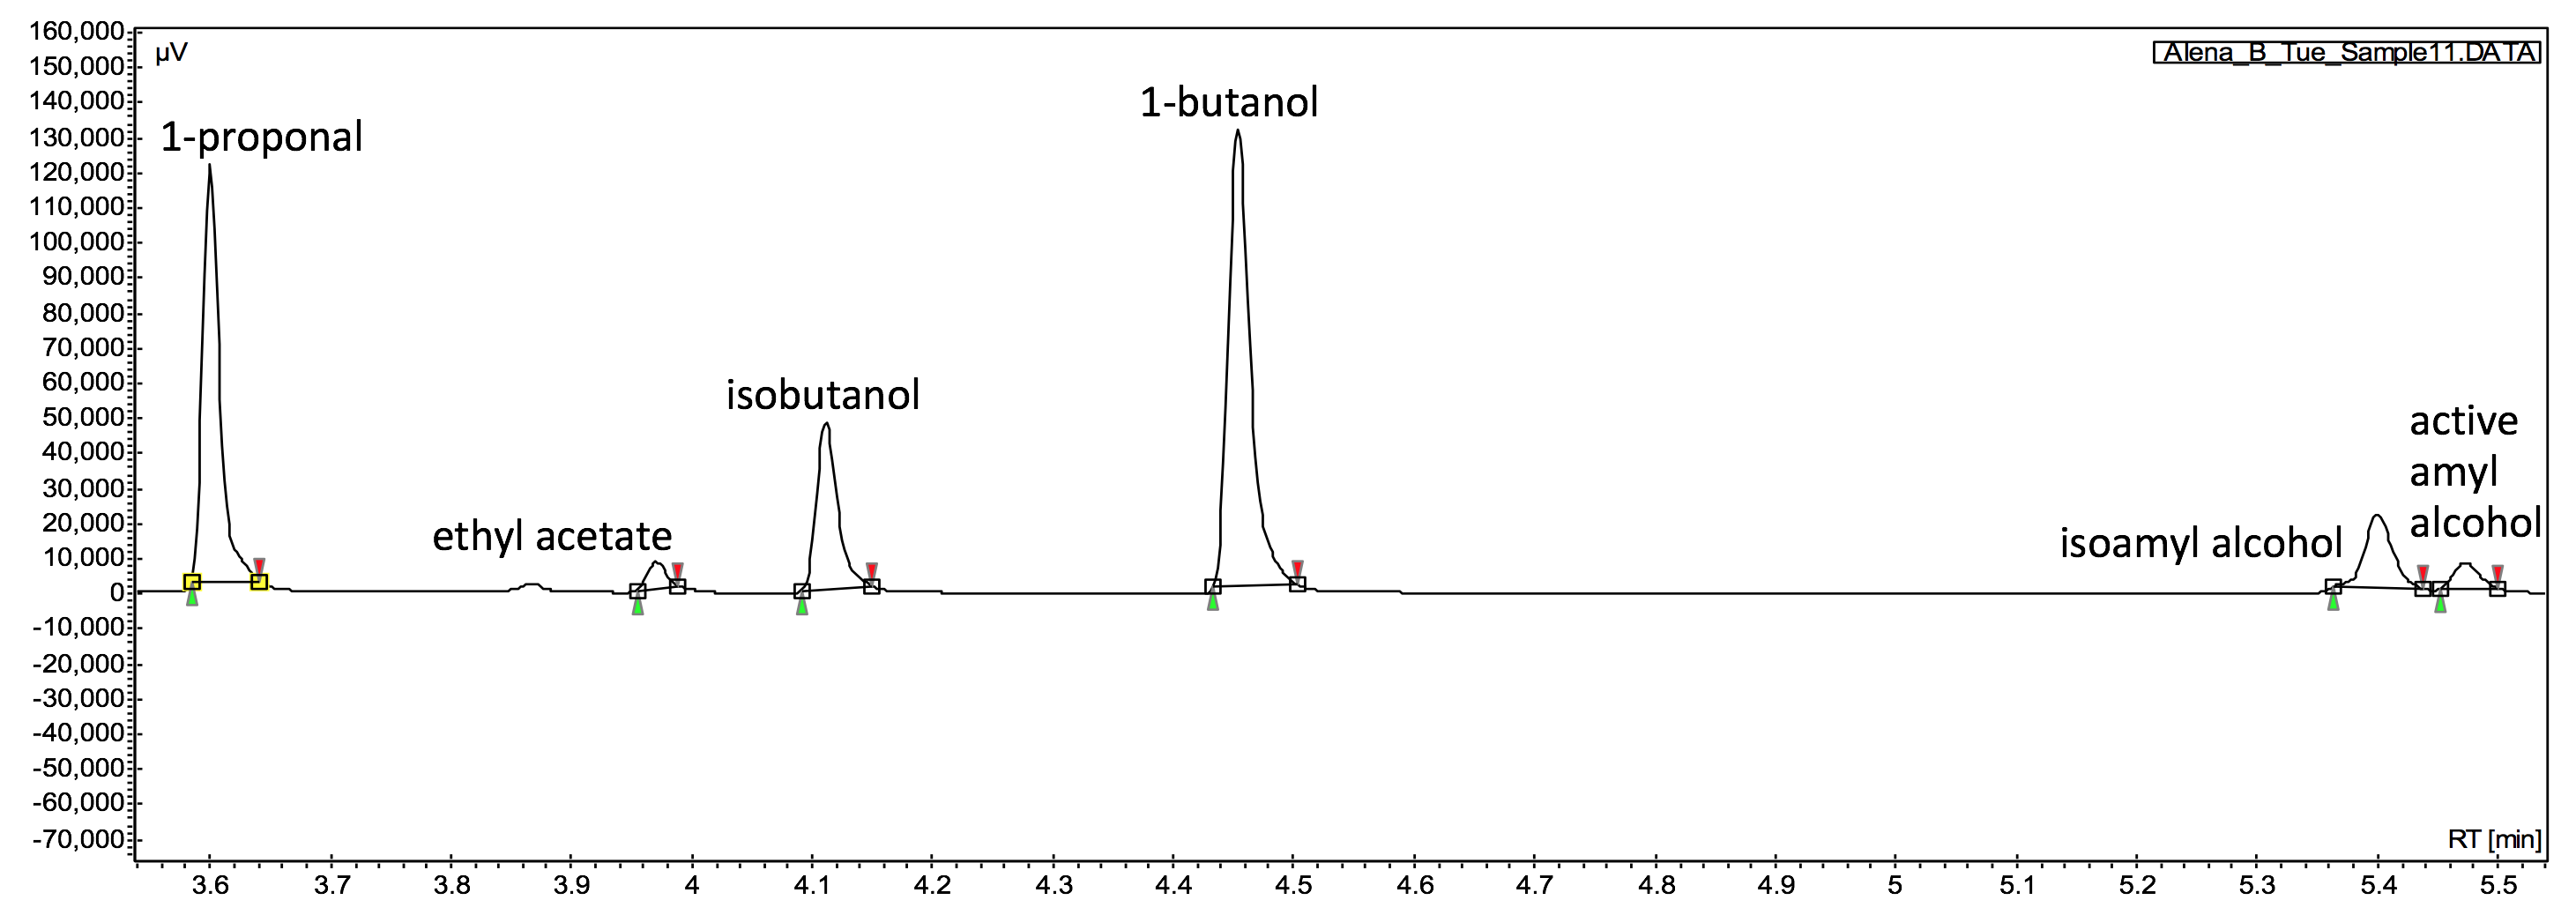
\includegraphics[scale=0.3]{sample1.png}
    \captionof{figure}{Chromatogram of spiked sample run 1.}

    \vspace{0.8cm}

	% Sample_2
    \captionof{table}{Whiskey sample chromatogram run 2.}
   \resizebox{0.9\textwidth}{!}{\begin{tabular}{lrrrrrrr}
   \textbf{Sample\_2} &   &   &   &   &   &   &  \\
   \# & \multicolumn{1}{l}{Name} & \multicolumn{1}{l}{Time [Min]} & \multicolumn{1}{l}{Quantity [\% Area]} & \multicolumn{1}{l}{Height [µV]} & \multicolumn{1}{l}{Area [µV.Min]} & \multicolumn{1}{l}{Area \% [\%]} & \multicolumn{1}{l}{Width 50\% [Min]} \\
       \hline
   \multicolumn{1}{r}{1} & \multicolumn{1}{l}{1-proponal} & 3.61 & 30.81 & 135123.9 & 2505.9 & 30.81 & 0.016 \\
   \multicolumn{1}{r}{2} & \multicolumn{1}{l}{ethyl acetate} & 3.97 & 2.01 & 7655.2 & 163.5 & 2.011 & 0.021 \\
   \multicolumn{1}{r}{3} & \multicolumn{1}{l}{isobutanol} & 4.12 & 12.73 & 49451.6 & 1035.4 & 12.731 & 0.019 \\
   \multicolumn{1}{r}{4} & \multicolumn{1}{l}{1-butanol} & 4.46 & 42.37 & 148710.9 & 3446.4 & 42.374 & 0.02 \\
   \multicolumn{1}{r}{5} & \multicolumn{1}{l}{isoamyl alcohol} & 5.41 & 9.32 & 25575.7 & 758 & 9.319 & 0.025 \\
   \multicolumn{1}{r}{6} & \multicolumn{1}{l}{active amyl alcohol} & 5.48 & 2.75 & 8702.7 & 224 & 2.754 & 0.025 \\
     &   &   &   &   &   &   &  \\
   Total &   &   & 100 & 375220.1 & 8133.2 & 100 &  \\
   \end{tabular}}

    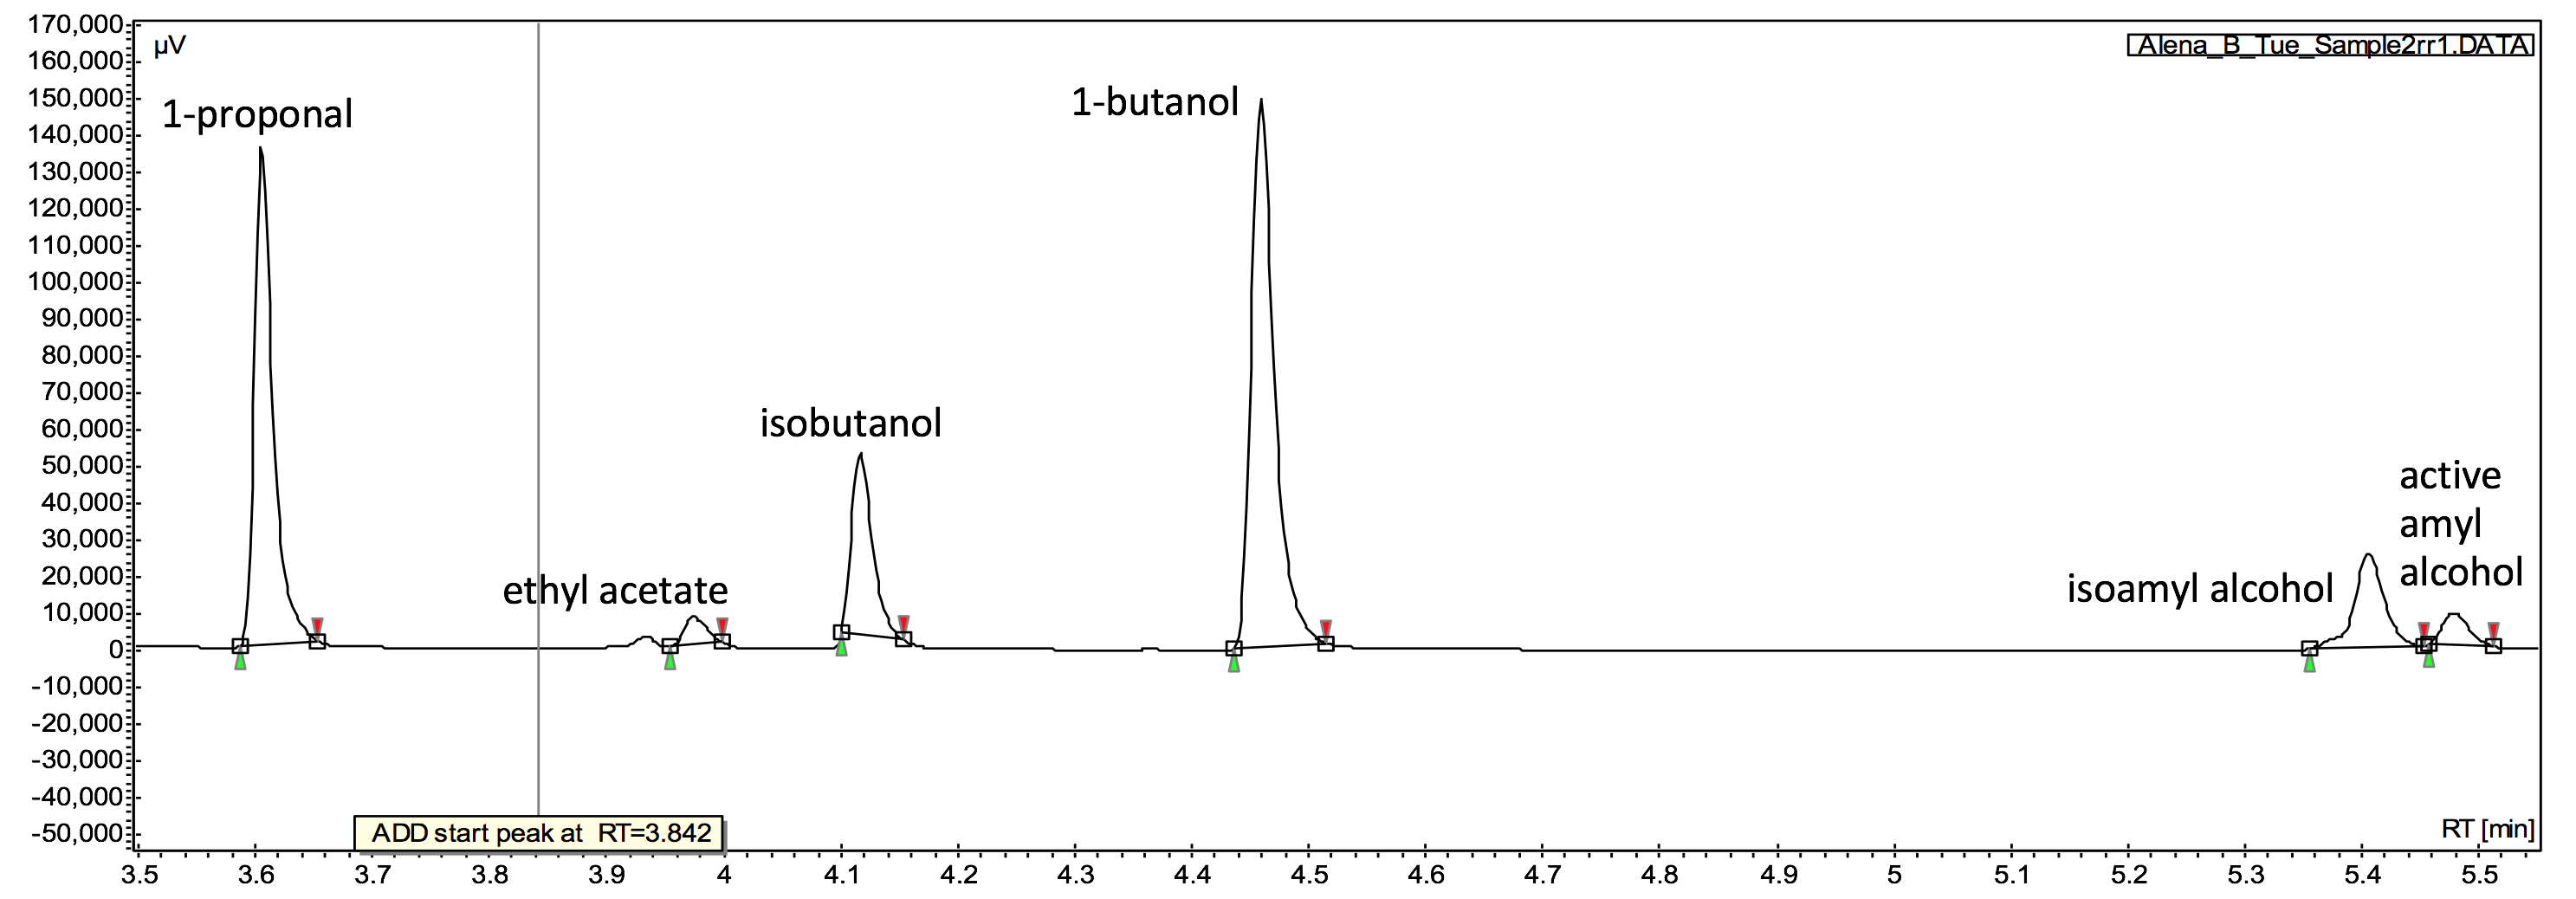
\includegraphics[scale=0.3]{sample2.png}
    \captionof{figure}{Chromatogram of spiked sample run 2.}

	% Sample_3
    \captionof{table}{Whiskey sample chromatogram run 3.}
   \resizebox{0.9\textwidth}{!}{\begin{tabular}{lrrrrrrr}
   \textbf{Sample\_3} &   &   &   &   &   &   &  \\
   \# & \multicolumn{1}{l}{Name} & \multicolumn{1}{l}{Time [Min]} & \multicolumn{1}{l}{Quantity [\% Area]} & \multicolumn{1}{l}{Height [µV]} & \multicolumn{1}{l}{Area [µV.Min]} & \multicolumn{1}{l}{Area \% [\%]} & \multicolumn{1}{l}{Width 50\% [Min]} \\
       \hline
   \multicolumn{1}{r}{1} & \multicolumn{1}{l}{1-proponal} & 3.6 & 29.86 & 116576.4 & 2207.6 & 29.857 & 0.017 \\
   \multicolumn{1}{r}{2} & \multicolumn{1}{l}{ethyl acetate} & 3.98 & 1.96 & 7131.7 & 145.1 & 1.963 & 0.02 \\
   \multicolumn{1}{r}{3} & \multicolumn{1}{l}{isobutanol} & 4.12 & 14.43 & 47661.4 & 1066.8 & 14.428 & 0.021 \\
   \multicolumn{1}{r}{4} & \multicolumn{1}{l}{1-butanol} & 4.46 & 42.36 & 132341.1 & 3131.8 & 42.356 & 0.021 \\
   \multicolumn{1}{r}{5} & \multicolumn{1}{l}{isoamyl alcohol} & 5.4 & 8.63 & 22314.1 & 638.4 & 8.635 & 0.026 \\
   \multicolumn{1}{r}{6} & \multicolumn{1}{l}{active amyl alcohol} & 5.48 & 2.76 & 7870.4 & 204.2 & 2.762 & 0.025 \\
     &   &   &   &   &   &   &  \\
   Total &   &   & 100 & 333895.1 & 7393.9 & 100 &  \\
   \end{tabular}}

    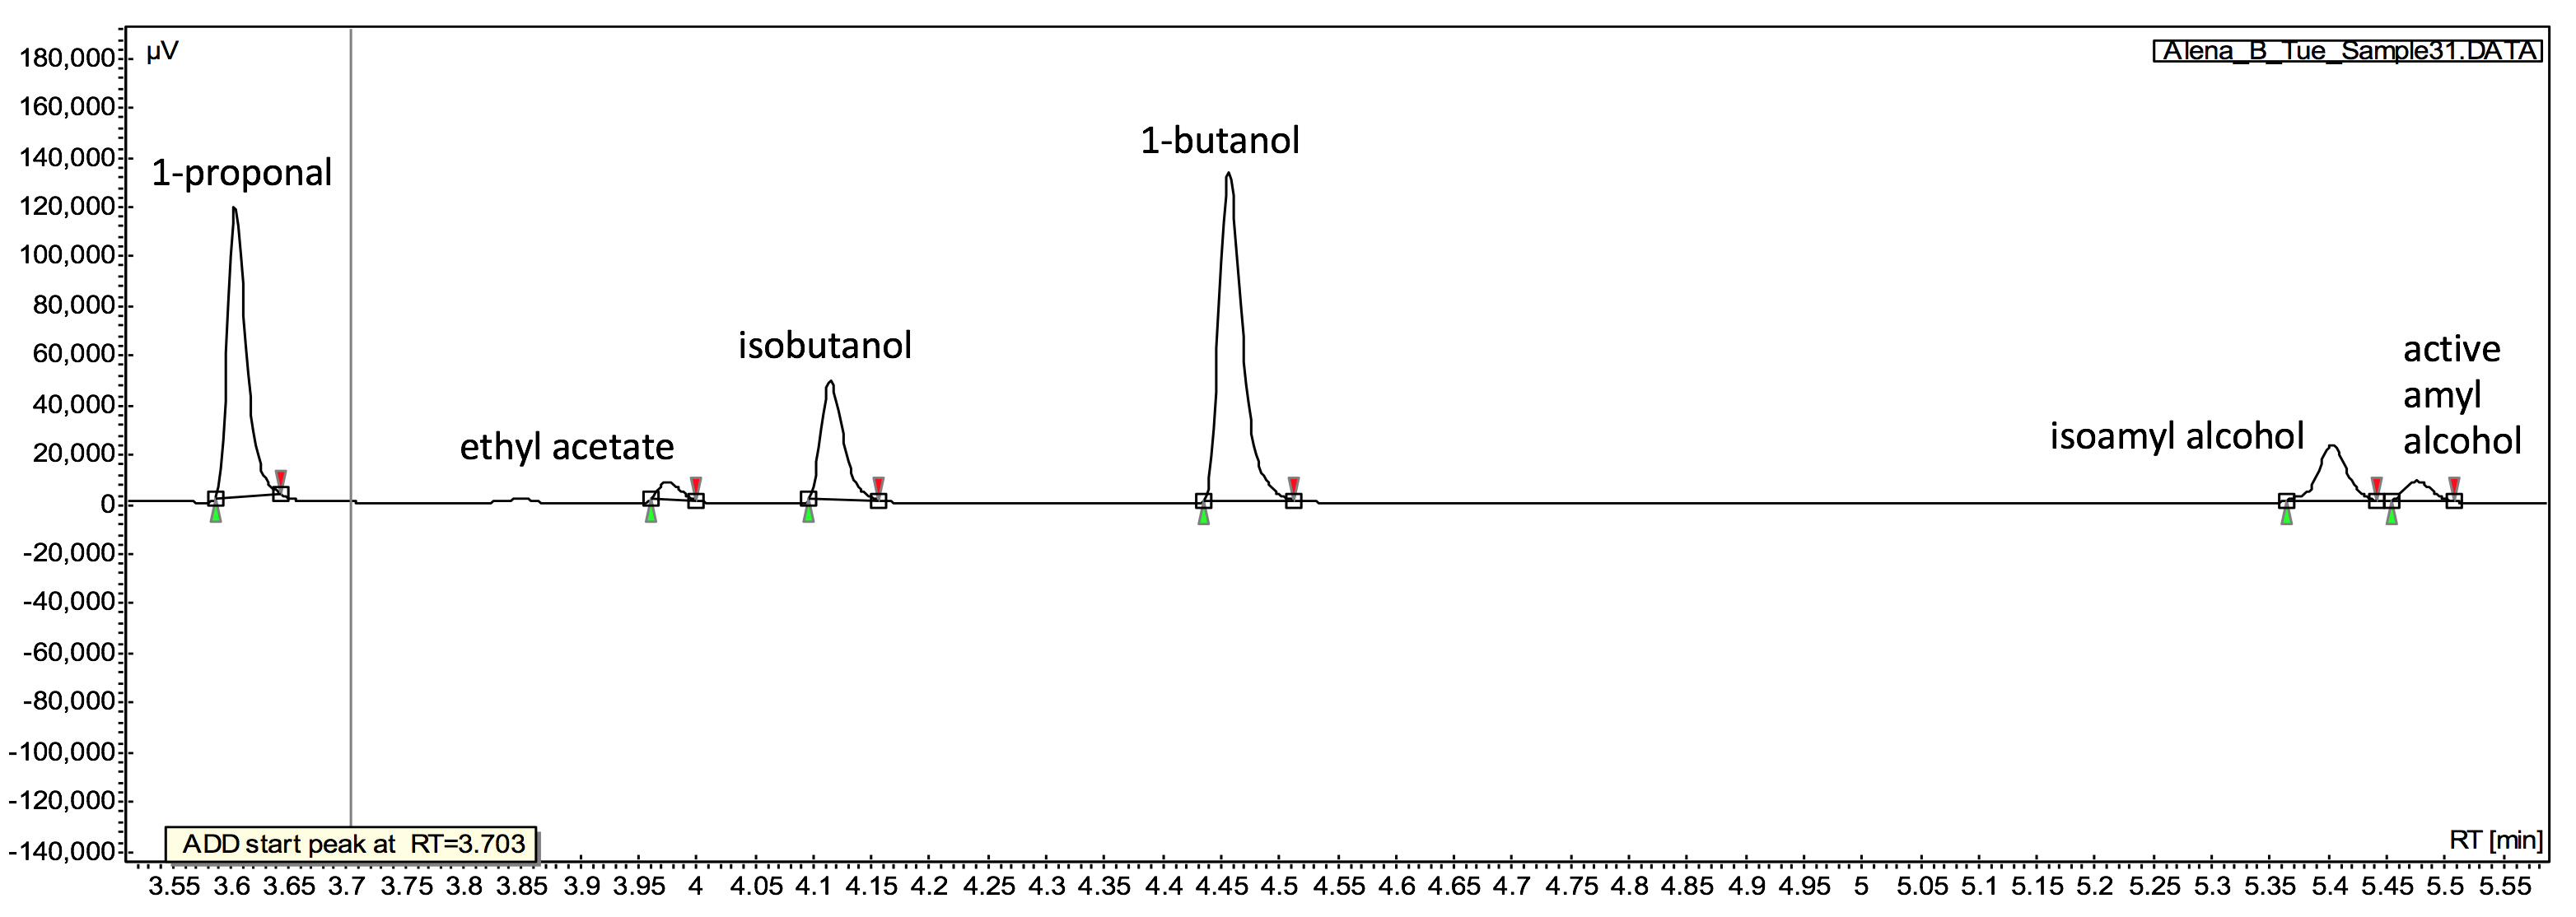
\includegraphics[scale=0.3]{sample3.png}
    \captionof{figure}{Chromatogram of spiked sample run 3.}

\newpage

	% Standard Retention Times 
    \captionof{table}{Retention times of standard solution (min).}
   \resizebox{0.7\textwidth}{!}{\begin{tabular}{lrrrr}
   %\textbf{} &   &   &   &  \\
   Alcohol & \multicolumn{1}{l}{standard 1} & \multicolumn{1}{l}{standard 2} &
       \multicolumn{1}{l}{standard 3} & \multicolumn{1}{l}{average retention
       time} \\
       \hline
   1-proponal & 3.6 & 3.6 & 3.6 & 3.6 \\
   ethyl acetate & 3.97 & 3.98 & 3.98 & 3.98 \\
   isobutanol & 4.11 & 4.11 & 4.11 & 4.11 \\
   1-butanol & 4.45 & 4.46 & 4.45 & 4.45 \\
   isoamyl alcohol & 5.39 & 5.4 & 5.4 & 5.4 \\
   active amyl alcohol & 5.47 & 5.47 & 5.47 & 5.47 \\
   \end{tabular}}

   \vspace{2cm}

	% Standard Peak Areas
    \captionof{table}{Peak areas of standard solution (µV$\times$min).}
   \resizebox{0.7\textwidth}{!}{\begin{tabular}{lrrrr}
       %\textbf{Standard Peak Areas (µV$\times$min)} &   & \multicolumn{1}{l}{} &   &  \\
   Alcohol & \multicolumn{1}{l}{standard 1} & \multicolumn{1}{l}{standard 2} &
       \multicolumn{1}{l}{standard 3} & \multicolumn{1}{l}{average peak area} \\
       \hline
   1-proponal & 1108.3 & 451.7 & 870.3 & 810.1 \\
   ethyl acetate & 769.1 & 342.3 & 610.1 & 573.8 \\
   isobutanol & 1189.9 & 497.9 & 987.8 & 891.9 \\
   1-butanol & 1297.4 & 533.2 & 1076.7 & 969.1 \\
   isoamyl alcohol & 1192.2 & 474.6 & 949.6 & 872.1 \\
   active amyl alcohol & 981.4 & 428.1 & 812.5 & 740.7 \\
   \end{tabular}}

   \vspace{2cm}

	% Standard Detector Response Factor
    \captionof{table}{Detector Response Factor of standard solution.}
   \resizebox{0.7\textwidth}{!}{\begin{tabular}{lrrrr}
   %\textbf{Standard Detector Response Factor} &   &   &   &  \\
   Alcohol & \multicolumn{1}{l}{standard 1} & \multicolumn{1}{l}{standard 2} &
       \multicolumn{1}{l}{standard 3} & \multicolumn{1}{l}{average response factor} \\
       \hline
   1-proponal & 0.85425 & 0.8472 & 0.8083 & 0.8366 \\
   ethyl acetate & 0.5928 & 0.6420 & 0.5666 & 0.6005 \\
   isobutanol & 0.91714 & 0.9338 & 0.9174 & 0.9228 \\
   isoamyl alcohol & 0.91892 & 0.8901 & 0.8820 & 0.8970 \\
   active amyl alcohol & 0.8232 & 0.9020 & 0.7546 & 0.8266 \\
   \end{tabular}}

   \vspace{2cm}

	% Sample Alcohol Concentration
    \captionof{table}{Concentration of whiskey sample components (ppm).}
   \resizebox{0.7\textwidth}{!}{\begin{tabular}{lrrrr}
       %\textbf{Sample Alcohol Concentration (ppm)} &   &   & \multicolumn{1}{l}{} &  \\
   Alcohol & \multicolumn{1}{l}{sample 1} & \multicolumn{1}{l}{sample 2} &
       \multicolumn{1}{l}{sample 3} & \multicolumn{1}{l}{average concentration} \\
       \hline
   1-proponal & 400 & 400 & 400 & 400 \\
   ethyl acetate & 40 & 40 & 40 & 40 \\ 
   isobutanol & 200 & 200 & 200 & 200 \\
   1-butanol & 500 & 500 & 500 & 500 \\
   isoamyl alcohol & 100 & 100 & 100 & 100 \\
   active amyl alcohol & 40 & 40 & 40 & 40 \\
   \end{tabular}}

   \newpage

	% Sample Width 50%
    \captionof{table}{Sample peak width at 50\% (min).}
   \resizebox{0.7\textwidth}{!}{\begin{tabular}{lrrrr}
   %\textbf{Sample Width 50\% (min)} &   &   &   &  \\
   Alcohol & \multicolumn{1}{l}{sample 1} & \multicolumn{1}{l}{sample 2} &
       \multicolumn{1}{l}{sample 3} & \multicolumn{1}{l}{average width 50\%} \\
       \hline
   1-proponal & 0.015 & 0.016 & 0.017 & 0.016 \\
   ethyl acetate & 0.017 & 0.021 & 0.02 & 0.02 \\
   isobutanol & 0.019 & 0.019 & 0.021 & 0.020 \\
   1-butanol & 0.019 & 0.02 & 0.021 & 0.02 \\
   isoamyl alcohol & 0.024 & 0.025 & 0.026 & 0.025 \\
   active amyl alcohol & 0.023 & 0.025 & 0.025 & 0.024 \\
   \end{tabular}}
   
   \vspace{2cm}

	% Sample Retension Time
    \captionof{table}{Retension time of sample (min).}
   \resizebox{0.7\textwidth}{!}{\begin{tabular}{lrrrr}
   %\textbf{Sample Retention Time (min)} &   &   &   &  \\
   Alcohol & \multicolumn{1}{l}{sample 1} & \multicolumn{1}{l}{sample 2} &
       \multicolumn{1}{l}{sample 3} & \multicolumn{1}{l}{average retention time} \\
       \hline
   1-proponal & 3.6 & 3.61 & 3.6 & 3.6 \\
   ethyl acetate & 3.97 & 3.97 & 3.98 & 3.97 \\
   isobutanol & 4.11 & 4.12 & 4.12 & 4.12 \\
   1-butanol & 4.45 & 4.46 & 4.46 & 4.46 \\
   isoamyl alcohol & 5.4 & 5.41 & 5.4 & 5.4 \\
   active amyl alcohol & 5.47 & 5.48 & 5.48 & 5.48 \\ 
   \end{tabular}}

   \vspace{2cm}

\begin{multicols}{2}
	% Number of Theoretical Plates
    \captionof{table}{Number of theoretical plates (N).}
   \resizebox{0.25\textwidth}{!}{\begin{tabular}{lr}
   %\textbf{Number of Theoretical Plates} &  \\
   Alcohol & \multicolumn{1}{l}{N} \\
       \hline
   1-proponal & 280000 \\
   ethyl acetate & 230000 \\
   isobutanol & 240000 \\
   1-butanol & 280000 \\
   isoamyl alcohol & 260000 \\
   active amyl alcohol & 280000 \\
   \end{tabular}}

   \vspace{1cm}

	% Height Equivelent to a Theoretical Plate
    \captionof{table}{Height equivalent to a theoretical plate.}
   \resizebox{0.3\textwidth}{!}{\begin{tabular}{lr}
   %\textbf{Height Equivalent to a Theoretical Plate} &  \\
   Alcohol & \multicolumn{1}{l}{HETP (mm)} \\
       \hline
   1-proponal & 0.2 \\
   ethyl acetate & 0.3 \\
   isobutanol & 0.2 \\
   1-butanol & 0.2 \\
   isoamyl alcohol & 0.2 \\
   active amyl alcohol & 0.2 \\
   \end{tabular}}

\end{multicols}

\newpage

\subsection*{Sample Calculations for Determining Concentration of 1-propanol}

\begin{align*} 
    \text{average retention time} &=  \frac{3.6 + 3.6 + 3.6}{3} \\ 
     &= 3.6\ min \\ 
\end{align*}

\begin{align*}
    \text{average area of peak} &= \frac{1108.3 + 451.7 + 870.3}{3} \\
     &= 810.1 \ \mu V\times min
\end{align*}

\begin{align*}
    \text{detector response factor} &= \frac{\textrm{area of peak$_{(1-propanol)}$ in standard}}
    {\textrm{area of peak$_{(1-butanol)}$ in standard}} \\
     &= \frac{1108.3}{1297.4} \\
     &= 0.85425
\end{align*}

\begin{align*}
    \text{[1-propanol]} &= \frac{\textrm{[1-butanol] $\times$ area of
    peak$_{(1-propanol)}$ in sample}}
    {\textrm{average detector response factor$_{(1-propanol)}$ $\times$ area of
    peak$_{(1-butanol)}$ in sample}} \\
     &= \frac{500 \times 1993.2}{0.83657 \times 2816.8} \\
     &= 400
\end{align*}

    %\sigma &= \sqrt{\frac{1}{N} }
    %\sum\limits_{i=1}^N (x_i - \mu)^2}

\begin{align*}
    \sigma_{[1-propanol]} &= \sqrt{\frac{1}{N}\sum\limits_{i=1}^N (x_i - \mu)^2} \\
    &= \sqrt{\frac{1}{3} \sum\limits_{i=1}^3 (0)^2} \\
    &= 0
\end{align*}

\end{center}
\end{document} 
